%-*- coding: utf-8 -*-
\label{chap:tests}

\paragraph{Notions :} hypothèse nulle, hypothèse alternative, statistique de
test, p-valeur, tests multiples.
\paragraph{Objectifs pédagogiques :} 
\begin{itemize}      
  \setlength{\itemsep}{3pt}
\item Reconnaître une situation dans laquelle un test statistique est
  approprié.
\item Poser les hypothèses de test nulle et alternative correspondant à un
  énoncé.
\item Interpréter une statistique de test ou une p-valeur.
\end{itemize}


\section{Principe d'un test statistique}
\label{sec:principe_test}
Le but d'un test statistique est de déterminer la fiabilité d'un résultat
obtenu sur un échantillon.

\begin{exemple}
Si je lance une pièce 5 fois et obtiens 5 fois pile, puis-je en déduire que
  la pièce est déséquilibrée ? Ou ce résultat est-il dû au hasard de
  l'échantillonnage ? Qu'en est-il si j'obtiens le même résultat après 50
  lancers ? 
\end{exemple}

\textbf{Un test statistique permet de déterminer si l'échantillon observé
  permet d'invalider une hypothèse qu'il était raisonnable de formuler avant
  d'observer les données.}

\begin{exemple}
  Reprenons l'exemple du lancer de pièce. Sous l'hypothèse que la pièce est
  équilibrée, la probabilité $\pi$ d'obtenir « pile » pour un lancer est $0,5$
  et celle d'obtenir pile pour 5 lancers est $0,5^5 = 3\%.$ Cette probabilité
  est faible, mais non négligeable : on a 3\% de chance d'obtenir un résultat
  aussi extrême que celui observé sur un échantillon.

  Pour 50 lancers, cette probabilité tombe à $0,5^{50} = 9 \cdot 10^{-16}.$
  Cette probabilité est extrêmement faible, et l'échantillon n'est pas cohérent
  avec l'hypothèse selon laquelle la pièce est équilibrée. Il est raisonnable
  de la rejeter.
\end{exemple}

\section{Formalisme}
\label{sec:formalisme_test}
Soit $(X_1, X_2, \dots, X_n)$ un échantillon aléatoire de taille $n \in \NN^*$
d'une variable aléatoire réelle $X$ de loi $\PP_X.$ Rappelons que les
composantes $X_i$ de ce vecteur aléatoire sont indépendantes et identiquement
distribuées, de même loi que $X$. Les notions présentées dans ce chapitre
s'appliquent aussi à des variables aléatoires de nature plus complexe (par
exemple, des valeurs aléatoires multi-dimensionnelles) mais nous nous limitons
aux variables aléatoires réelles par souci de simplicité.
Nous supposons aussi disposer d'un échantillon $(x_1, x_2, \dots, x_n)$ qui est
une réalisation de $(X_1, X_2, \dots, X_n)$.

Un test statistique repose sur les éléments suivants :
\begin{itemize}
\item Une \textbf{hypothèse nulle,} notée $\HH_0$. L'hypothèse nulle est
  celle que l'on cherche à rejeter.
\item Une \textbf{hypothèse alternative,} notée $\HH_1$ ou $\HH_a$. C'est en
  général la négation de $\HH_0$.
\item Une \textbf{statistique de test,} $T$, qui sert à mesurer à quel point un
  échantillon « dévie » de l'hypothèse nulle.
\item Un \textbf{niveau de signification,} $0 < \alpha < 1$, qui est la
  probabilité de rejeter l'hypothèse nulle alors qu'elle est correcte. 
% qui sert à
  % déterminer si la probabilité d'observer, sous $\HH_0$, une statistique de
  % test au moins aussi extrême que celle observée sur l'échantillon
  % $(x_1, x_2, \dots, x_n)$ est suffisamment faible pour rejeter $\HH_0$.
\end{itemize}

Le but de cette section est de développer ces notions.

\subsection{Hypothèses de test}
Conduire un test d'hypothèse nécessite de formuler deux hypothèses :
\begin{itemize}
\item Une \textbf{hypothèse nulle,} notée $\HH_0$. Cette hypothèse doit être
  précise et permettre de faire des calculs. Le but du test est de déterminer
  s'il est raisonnable de rejeter cette hypothèse.
\item Une \textbf{hypothèse alternative,} notée $\HH_1$ ou $\HH_a$. Cette
  hypothèse est une forme de négation de $\HH_0$, et c'est l'hypothèse que l'on
  adoptera si l'hypothèse nulle est rejetée.
\end{itemize}

L'hypothèse nulle est souvent une hypothèse formulée sur la valeur d'un paramètre
$\theta \in \Scal \subseteq \RR$ caractérisant la loi $\PP_X$ de l'échantillon
aléatoire. Il s'agit alors de tester
\begin{equation}
  \label{eq:h0}
  \HH_0: \theta = \theta_0,
\end{equation}
où $\theta_0 \in \Scal$ est une valeur déterministe fixée à l'avance.

L'hypothèse nulle peut cependant être de nature plus complexe, par exemple :
\begin{itemize}
\item « Deux variables statistique $X$ et $Y$ sont indépendantes » (c'est le
  cas du test d'indépendance du $\chi^2$ que nous verrons dans la PC1);
\item « Deux échantillons $(x_1, x_2, \dots, x_n)$ et $(y_1, y_2, \dots, y_n)$
  sont des réalisations de la même distribution » (c'est le cas du test de
  Wilcoxon-Mann-Whitney, qui dépasse le cadre de ce programme).
\end{itemize}

\paragraph{Présomption d'innocence} De même que le principe de la présomption
d'innocence veut que l'on recueille suffisamment de preuves pour rejeter
l'innocence d'une personne accusée, en théorie des tests statistiques il y a
présomption de $\HH_0$. Il s'agit donc de savoir si l'échantillon observé (les
preuves) est suffisant pour rejeter $\HH_0$, ce dont on conclura $\HH_1.$ Par
contre, si l'on ne rejette pas $\HH_0$, cela peut venir soit de ce que $\HH_0$
est vraie, soit de ce que nous n'avons pas suffisamment de données pour rejeter
$\HH_0$. Ainsi, $\HH_0$ doit être une hypothèse raisonnable, mais que l'on
aimerait avoir des raisons de réfuter.

Dans le cadre d'une expérience scientifique, l'hypothèse $\HH_0$ correspond
ainsi à l'état actuel des connaissances. Le but d'un test statistique est de
déterminer si les données qui semblent contredire cette hypothèse sont
effectivement suffisamment improbables sous $\HH_0$ pour justifier de la
réfuter.
Dans le cadre d'un essai clinique, par exemple, l'hypothèse $\HH_0$ se doit
d'être défavorable au nouveau médicament (« le nouveau médicament est
inefficace » ou « le nouveau médicament n'est pas plus efficace que les
traitements connus »). Le but du test statistique est de déterminer si les
données récoltées jusqu'à présent sont suffisantes pour réfuter cette
hypothèse.

\begin{exemple}
  Dans le cas de notre lancer de pièce,
  \begin{itemize}
  \item $X$ est une variable aléatoire discrète qui suit une loi de Bernoulli
    de paramètre $\pi$ ;
  \item l'échantillon aléatoire est un vecteur $(X_1, X_2, \dots, X_n)$ de $n$
    composantes, iid de même loi que $X$ ;
  \item une série de lancers est une réalisation $(x_1, x_2, \dots, x_n)$ de ce
    vecteur aléatoire. Dans le cas de 5 lancers tous tombant sur « pile »,
    cet échantillon est $(1, 1, 1, 1, 1)$ et $n=5.$
  \item l'hypothèse nulle est $\HH_0: \pi = 0,5.$
  \end{itemize}
\end{exemple}

Dans le cas où l'on cherche à tester la valeur d'un paramètre $\theta$ d'une
population, l'hypothèse alternative peut prendre deux formes :
\begin{itemize}
\item $\theta \neq \theta_0$, ou en d'autres termes, 
  \begin{equation}
    \label{eq:h1_bilateral}
    \HH_1: \theta < \theta_0 \text{ ou } \theta > \theta_0.
  \end{equation}
  On parle alors de test \textbf{bilatéral} (\textit{two-sided test} en
  anglais).
\item Si seulement l'une des deux parties de cette hypothèse alternative nous
  intéresse, ou est possible, on parle de test \textbf{unilatéral}
  (\textit{one-sided test} en anglais). Il s'agit alors de tester soit
  \begin{equation}
    \label{eq:h1_unilateral_gauche}
    \HH_1: \theta < \theta_0,
  \end{equation}
  soit
  \begin{equation}
    \label{eq:h1_unilateral_droite}
    \HH_1:  \theta > \theta_0.
  \end{equation}
\end{itemize}

De même que l'on élabore $\HH_0$ de sorte à ce qu'elle soit la plus plausible
avant d'avoir observé les données, on élabore $\HH_1$ en fonction de ce que
l'on espère découvrir. 

Reprenons l'exemple d'un essai clinique sur un nouveau médicament. Si
l'hypothèse $\HH_0$ est « le nouveau médicament n'a pas d'effet », on peut
poser l'hypothèse alternative $\HH_1$ : « le nouveau traitement a un effet
positif sur l'état des patients ». On espère ici non seulement rejeter
l'hypothèse nulle, mais aussi suggérer une efficacité du traitement. Cette
hypothèse est plus précise que l'hypothèse alternative selon laquelle « le
nouveau traitement a un effet sur l'état des patients », cet effet pouvant être
négatif.

\begin{exemple}
  Dans le cas de notre lancer de pièce, l'hypothèse alternative dans le cadre
  d'un test bilatéral est
  \[
    \HH_1: \pi \neq 0,5.
  \]
  Si nous rejetons $\HH_0,$ notre conclusion sera que la pièce n'est pas équilibrée.

  Dans le cadre d'un test unilatéral, par exemple
  \[
    \HH_1: \pi > 0,5,
  \]
  si nous rejetons $\HH_0,$ notre conclusion sera que la pièce n'est pas
  équilibrée, et qu'elle favorise « pile ».

  Il ne s'agit donc pas du même test.
\end{exemple}


\subsection{Statistique de test}
Une \textbf{statistique de test} $T$ est une statistique de l'échantillon
aléatoire. Il s'agit donc d'une variable aléatoire réelle, fonction de
$(X_1, X_2, \dots, X_n) : T = g(X_1, X_2, \dots, X_n)$. Cette statistique de
test sert à mesurer à quel point un échantillon « dévie » de l'hypothèse nulle.

Une statistique de test est ainsi choisie de sorte à avoir une loi différente
sous $\HH_0$ et sous $\HH_1$, et de sorte à ce que sa loi sous $\HH_0$ soit
connue : c'est ce qui permettra de déterminer un critère de rejet de $\HH_0$
garantissant le niveau de signification choisi.

La plupart des test statistiques reposent sur des statistiques de test dont le
développement a été long et minutieux. Le choix entre plusieurs statistiques
candidates pour un même problème est un choix difficile, qui repose entre
autres sur la validité des hypothèses sur la distribution de l'échantillon
aléatoire ou sur sa taille qui permettent de déterminer sa loi sous $\HH_0$.

\paragraph{Remarque} Pour des tests portant sur un paramètre
($\HH_0: \theta = \theta_0$), la statistique de test est souvent basée sur la
différence entre un estimateur de ce paramètre et sa valeur sous $\HH_0$.

\begin{exemple}
  Reprenons l'exemple du lancer de pièce.

  Dans la section~\ref{sec:principe_test}, nous avons choisi comme statistique
  de test $T$ le nombre de «~pile~» obtenus dans l'échantillon :
  \[
    T = \sum_{i=1}^n X_i.
  \]

  Sous $\HH_0$, autrement dit si $\pi=0,5$, la loi de $T$ est déterminée par 
  \[
    \PP(T=k) = \PP\left(\sum_{i=1}^n X_i = k\right) \text{ pour } k=0, 1,
    \dots, n.
  \]
  On reconnait ici une loi binomiale de paramètres $n$ et $\pi.$
\end{exemple}


\subsection{Niveau de signification}
Nous avons maintenant posé $\HH_0$, $\HH_1$, et une statistique de test $T$
dont nous connaissons la loi $\PP_{T0}$ sous $\HH_0$. Il nous faut maintenant
déterminer le \textbf{domaine de rejet} du test, autrement dit l'ensemble
$\Ical \subseteq \RR$ de ses valeurs qui conduisent à rejeter $\HH_0$.

Pour ce faire, nous avons besoin de fixer le \textbf{niveau de signification}
(\textit{significance level}), $0 < \alpha < 1$, qui est la probabilité de
rejeter l'hypothèse nulle alors qu'elle est correcte. Ce seuil est fixé à
l'avance, généralement parmi $\alpha = 1\%$, $\alpha = 5\%$ ou $\alpha = 10\%$,
et détermine à quel point le test est strict.

Ainsi, il s'agit de déterminer $\Ical \subseteq \RR$ de sorte à ce que
$\PP_{T0}(T \in \Ical) = \alpha.$

\begin{exemple}
  Dans l'exemple du lancer de pièce, nous avons choisi le nombre de «~pile~» comme
  statistique de test $T$. Sous $\HH_0 : \pi = 0,5$, $T$ suit une loi binomiale
  de paramètres $n$ (le nombre de lancers) et $\pi$.

  Posons $\alpha = 5\%.$

  Considérons le test unilatéral $\HH_1 : \pi > 0,5$. Si nous rejetons $\HH_0$,
  nous en conclurons que la pièce est biaisée en faveur du côté pile. Cela
  signifie que nous souhaitons rejeter $\HH_0$ quand le nombre de «~pile~» dans
  l'échantillon est grand. Il est ici naturel de considérer un domaine de rejet
  de la forme $\Ical = \mathopen]t_0, n\mathclose].$ En d'autres termes, nous
  allons rejeter $\HH_0$ si la réalisation $t$ de $T$ sur notre échantillon est
  plus grande qu'un seuil $t_0,$ fixé tel que $\PP_{T0}(T > t_0) = \alpha.$

  Appelons $F_{T0}$ la fonction de répartition de $T$ sous $\HH_0.$ Alors $t_0$
  est fixé de sorte à ce que $F_{T0}(t_0) = 1-\alpha$. Dans notre exemple avec
  $n=5$ et $\alpha=0,05$, cela fixe $t_0 = 4.$

  Le test consiste donc à rejeter l'hypothèse nulle si tous les 5 lancers
  aboutissent à pile.

  Considérons maintenant le test unilatéral $\HH_1 : \pi < 0,5.$ Rejeter
  $\HH_0$ conduit à conclure que la pièce est biaisée en faveur du côté
  face. Nous considérons maintenant un domaine de rejet de la forme
  $\Ical = \mathopen[0, t_0 \mathclose[,$ et $t_0$ est déterminé par
  $\PP_{T0}(T < t_0) = \alpha.$ Avec $n=5$ et $\alpha=0,05$, cela fixe
  $t_0=1$. Le test consiste donc à rejeter l'hypothèse nulle si aucun des 5
  lancers n'aboutit à pile.

  Enfin, considérons le test bilatéral $\HH_1 : \pi \neq 0,5.$ Rejeter $\HH_0$
  conduit à conclure que la pièce est biaisée, en faveur de l'un ou de l'autre
  de ses côtés. Nous considérons alors un domaine de rejet de la forme
  $\Ical = \mathopen[0, t_l \mathclose[ \; \cup \; \mathopen]t_r, n
  \mathclose].$
  Il nous faut donc choisir $t_l$ et $t_r$ de sorte à ce que
  $\PP_{T0}(T < t_l) + \PP_{T0}(T > t_r) = \alpha.$ Il est assez naturel de
  fixer alors $\PP_{T0}(T < t_l) = \PP_{T0}(T > t_r) = \frac{\alpha}{2}.$ Avec
  $n=5$ et $\alpha=0,05$, on obtient $t_l = 0$ et $t_r = 5$ et il n'est donc
  jamais possible de rejeter l'hypothèse nulle.

  Le test que nous venons de définir s'appelle le \textbf{test binomial.}

  \paragraph{Remarque importante} On observe ici que, parmi les trois
  hypothèses alternatives envisagées, seul le test statistique unilatéral
  $\HH_1: \pi > 0,5$ nous permet de rejeter l'hypothèse nulle. C'est une
  observation générale : un test unilatéral est plus puissant qu'un test
  bilatéral ; cependant il n'est utile que si on sait de quel côté le définir.
\end{exemple}

\subsection{Valeur critique}
Dans le cas d'un test sur la valeur d'un paramètre $\theta$, c'est-à-dire avec
pour hypothèse nulle 
\[
  \HH_0: \theta = \theta_0,
\]
le domaine de rejet sera de la forme
\begin{itemize}
\item $\Ical = \mathopen]t_r, +\infty \mathclose[$ pour le test unilatéral à
  droite, pour lequel $\HH_1 : \theta > \theta_0$ ;
\item $\Ical = \mathopen]-\infty, t_l \mathclose[$ pour le test unilatéral à
  gauche, pour lequel $\HH_1 : \theta > \theta_0$ ;
\item
  $\Ical = \mathopen]-\infty, t_l \mathclose[ \cup \mathopen]t_r, +\infty
  \mathclose[$
  pour le test bilatéral, pour lequel $\HH_1 : \theta \neq \theta_0$.
\end{itemize}

On utilisera le plus souvent une statistique de test symétrique, de sorte à
ce que $t_r = - t_l$.  Dans ce cas $t_0 = t_r$ est appelée
\textbf{valeur critique} du test et est telle que
\begin{itemize}
\item $\PP_{T0}(T > t_0) = \alpha$ pour le test unilatéral à droite ; 
\item $\PP_{T0}(T < - t_0) = \alpha$ pour le test unilatéral à gauche ; 
\item $\PP_{T0}(|T| > t_0) = \alpha$ pour le test bilatéral. 
\end{itemize}

\subsection{p-valeur}
La \textbf{p-valeur} (\textit{p-value} en anglais) d'un test statistique est
définie dans le cas où le test statistique peut être réalisé en comparant une
statistique de test $T$% \footnote{ou sa valeur absolue $\abs{T}$, sans perte de
  % généralité, puisque l'on peut alors utiliser la statistique $U = \abs{T}.$}
à
une valeur critique $t_0$.

Dans ce contexte, étant donné un échantillon $(x_1, x_2, \dots, x_n)$ et la
réalisation $t$ de $T$ sur cet échantillon, on appelle \textbf{p-valeur} la
probabilité $\PP_{T0}(T > t)$ pour un test unilatéral à droite (respectivement,
$\PP_{T0}(T < -t)$ pour un test unilatéral à gauche, et $\PP_{T0}(\abs{T} > t)$
pour un test bilatéral). 

L'hypothèse nulle est rejetée si la p-valeur est plus petite que le niveau de
signification. On dit alors que la p-valeur est \textbf{significative.}

En d'autres termes, la p-valeur peut être interprétée comme la probabilité
d'obtenir, sous l'hypothèse nulle, un résultat au moins aussi extrême que celui
observé.

On rapporte ainsi généralement comme résultat d'un test non pas la réalisation
de la statistique de test sur l'échantillon observé, mais la p-valeur
correspondante.

On lira ainsi dans des publications scientifiques des assertions suivies de «
($p < 0,05$) », signifiant que l'assertion en question est l'hypothèse
alternative d'un test dont l'hypothèse nulle a été rejetée avec une p-valeur
inférieure à $5\%.$

\begin{attention}
  On fera attention à ne pas sur-interpréter la p-valeur. En particulier, la
  p-valeur \textit{n'est pas} la probabilité que l'hypothèse nulle soit vraie :
  $\PP(t|\HH_0) \neq \PP(\HH_0|t)$.
\end{attention}

\newpage
\begin{exemple}
  Le test que nous avons défini dans l'exemple de la pièce de monnaie s'appelle
  le test binomial. Il est implémenté dans \texttt{scipy.stats} :
  \begin{lstlisting}[language=Python]
    t = 5 # nb pile 
    n = 5 # taille échantillons 
    pi = 0.5 
    import scipy.stats as st 
    st.binom_test(t, n, pi, alternative='greater') # unilatéral à droite
  \end{lstlisting}
\end{exemple}



\subsection{Erreurs de première et deuxième espèce $\bullet$}
\label{sec:test_errors}
Deux types d'erreurs sont possibles quand on fait un test d'hypothèse :
\begin{itemize}
\item Rejeter l'hypothèse nulle alors qu'elle est correcte : on parle d'une
  \textbf{erreur de première espèce}, ou \textbf{erreur de Type I}
  (\textit{Type I error} en anglais).
\item Accepter l'hypothèse nulle alors qu'elle est en fait fausse : on parle
  d'une \textbf{erreur de deuxième espèce}, ou \textbf{erreur de Type II}
  (\textit{Type II error} en anglais).
\end{itemize}

\paragraph{Moyen mnémotechnique} Ces deux types d'erreurs sont numérotés dans
le même ordre que dans l'histoire du garçon qui criait au loup : d'abord les
villageois pensaient qu'il y avait un loup alors qu'il n'y en avait pas (erreur
de première espèce), mais à la fin les villageois pensaient qu'il n'y avait pas
de loup alors qu'il y en avait un (erreur de deuxième espèce). Ici, l'hypothèse
nulle est l'hypothèse correspondant à l'état « par défaut » du village, à
savoir sans loup\footnote{Les fans de \textit{Battlestar Galactica} pourront
construire leur propre moyen mnémotechnique à partir de Starbuck qui refuse
de faire valider les élèves pilotes après avoir fait valider Zak.}.

Le niveau de signification $\alpha$ est ainsi la probabilité de commettre une
erreur de première espèce.

La probabilité de commettre une erreur de deuxième espèce est généralement noté
$\beta$. La probabilité de rejeter $\HH_0$ à raison, $1-\beta$, est appelée la
\textbf{puissance} du test (\textit{power} en anglais).


\section{Comparaison d'une moyenne observée à une moyenne théorique}
\label{sec:test_moyenne}
Dans cette section, nous allons dérouler un autre exemple de test statistique. 

Nous souhaitons tester l'hypothèse selon laquelle les pigeons du Jardin du
Luxembourg ont un poids moyen de 300g. Nous disposons de mesures pour 40
pigeons, capturés et pesés par des élèves de l'École, dont la moyenne est de
312g et l'écart-type 31g.

Définissons une variable aléatoire réelle $X$ de carré intégrable. $X$ modélise
le poids d'un pigeon. Posons $\mu$ l'espérance de $X$ et $\sigma^2$ sa
variance.

\subsection{Hypothèses de test}
\paragraph{Question:} Comment modéliser ce problème ? Que poser pour $\HH_0$ et
$\HH_1$ ? \newpage
\begin{answer}
  Nous posons $n=40$ ; les poids des 40 pigeons, $(x_1, x_2, \dots, x_n)$, sont
  la réalisation de l'échantillon aléatoire $(X_1, X_2, \dots, X_n)$ composé de
  variables aléatoires indépendantes et identiquement distribuées de même loi
  que $X$.

  Nous posons l'hypothèse nulle à tester
  \[
    \HH_0 : \mu = \mu_0,
  \]
  avec $\mu_0 = 300\si{g}.$

  Nous n'avons aucun a priori sur le poids des pigeons du Jardin du Luxembourg,
  et formulons donc l'hypothèse alternative bilatérale
  \[
    \HH_1 : \mu \neq \mu_0.
  \]
\end{answer}

\subsection{Statistique de test}
Pour tester $\HH_0$, nous souhaitons déterminer la probabilité d'observer une
moyenne empirique $\hatm$ de 312g si l'espérance de $X$ est de 300g.  En
posant $M_n$ la moyenne empirique de l'échantillon, nous souhaitons déterminer
$\PP(M_n=\hatm|\mu=\mu_0)$.

Le théorème central limite nous indique que 
\[
  \frac{\sqrt{n} (M_n - \mu)}{\sigma}  \cvloi \Ncal(0, 1).
\]

Avec $n = 40$, nous pouvons supposer que cette limite est suffisamment proche
d'être atteinte pour poser
\[
  \frac{\sqrt{n} (M_n - \mu)}{\sigma}  \sim \Ncal(0, 1).
\]

Nous ne connaissons pas la variance $\sigma^2$ de $X$ ; cependant nous pouvons
l'estimer grâce à l'écart-type empirique $\hatsigma = 31\si{g},$ et utiliser 
\begin{equation}
  \frac{\sqrt{n} (M_n - \mu)}{\hatsigma}  \sim \Ncal(0, 1).
\label{eq:tcl_moyenne}
\end{equation}
Nous ne remplaçons pas $\mu$ par son estimation $\hatm$ : ce n'aurait aucun
sens, car nous cherchons justement à tester sa valeur.

\paragraph{Question :} Comment utiliser l'équation~\eqref{eq:tcl_moyenne} pour
définir une statistique de test ?
\begin{answer}
  Si $\HH_0$ est vraie, alors $\mu = \mu_0$ et la variable aléatoire réelle
  \begin{equation}
    \label{eq:z_moyennes}
    Z = \frac{\sqrt{n} (M_n - \mu_0)}{\hatsigma}
  \end{equation}
  est une gaussienne standard : $Z \sim \Ncal(0, 1)$.

  $Z$ est donc une variable aléatoire réelle dont nous connaissons la
  distribution sous l'hypothèse nulle. Cela en fait une bonne candidate à être
  statistique de test.
\end{answer}
Sous $\HH_0$, on s'attend à ce que la réalisation de $Z$ sur l'échantillon
observé soit proche de $0.$ Nous réalisons un test bilatéral et n'avons aucun a
priori sur le signe de $Z.$ Ainsi, nous rejetterons $\HH_0$ si la réalisation
de $\abs{Z}$ est « trop grande » pour être plausible.

Le test statistique permettant de tester si la moyenne d'un échantillon vaut
une valeur prédéterminée consiste donc à rejeter $\HH_0$ si $\abs{Z} > z_0.$

\paragraph{Question : } Étant donné un niveau de signification $\alpha$, quelle
est la valeur critique $z_0$ ?
\begin{answer}
  Nous souhaitons que la probabilité de rejeter $\HH_0$ alors qu'elle est vraie
  soit égale à $\alpha.$ En d'autres termes, nous cherchons $z_0$ tel que
  \[
    \PP(\abs{Z} > z_0) = \alpha, \text{ sachant } Z \sim \Ncal(0, 1).
  \]
  La densité de $Z$ étant symmétrique, on cherche donc $z_0$ telle que 
  \[
    \PP(Z < -z_0) = \frac{\alpha}{2}.
  \]
  Ceci est illustré sur la figure~\ref{fig:z_moyenne}.  
\end{answer}

\begin{figure}[h]
  \centering
  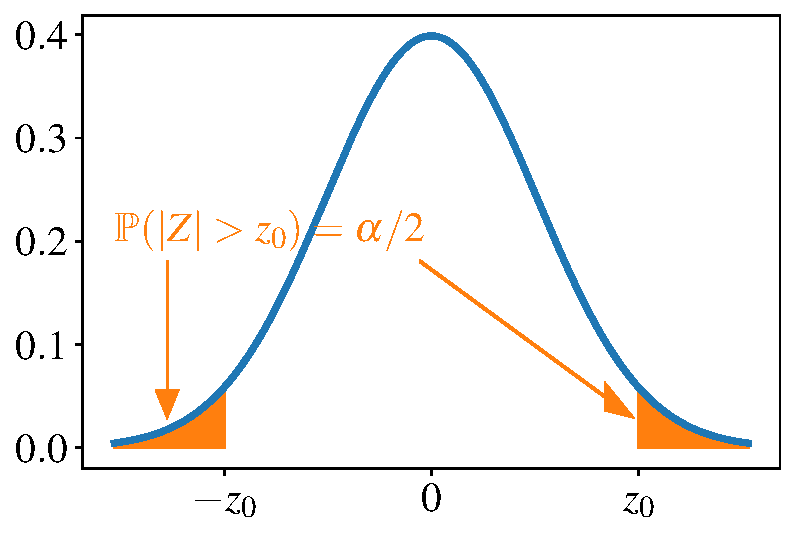
\includegraphics[width=0.5\textwidth]{figures/tests/z_moyenne}
  \caption{Densité d'une gaussienne centrée réduite. L'aire colorée vaut
    $\alpha$ et correspond au domaine de rejet du test.}
  \label{fig:z_moyenne}
\end{figure}

\paragraph{Question :} Peut-on rejeter l'hypothèse selon laquelle les pigeons
du jardin du Luxembourg ont un poids moyen de 300g ?
\begin{answer}
  Cela dépend du niveau de signification que l'on choisit.

  Calculons tout d'abord la réalisation de la statistique de test $Z$ sur notre
  échantillon : $z = 2,45.$

  Posons $\alpha = 0,05.$ Alors $z_0 \approx 1,96.$ On a bien $z > z_0$ et on
  rejette l'hypothèse nulle. On dit que l'écart entre $M_n$ et $\mu_0$ est
  \textbf{statistiquement significatif.}

  Posons maintenant $\alpha = 0,01.$ Le domaine de rejet est plus restreint ;
  $z_0 \approx 2,58.$ On ne peut pas rejeter l'hypothèse nulle. L'écart entre
  $M_n$ et $\mu_0$ n'est pas statistiquement significatif.


  Cet exemple est illustré sur la figure~\ref{fig:z_pigeons}.
\end{answer}


\begin{figure}[h]
  \centering
  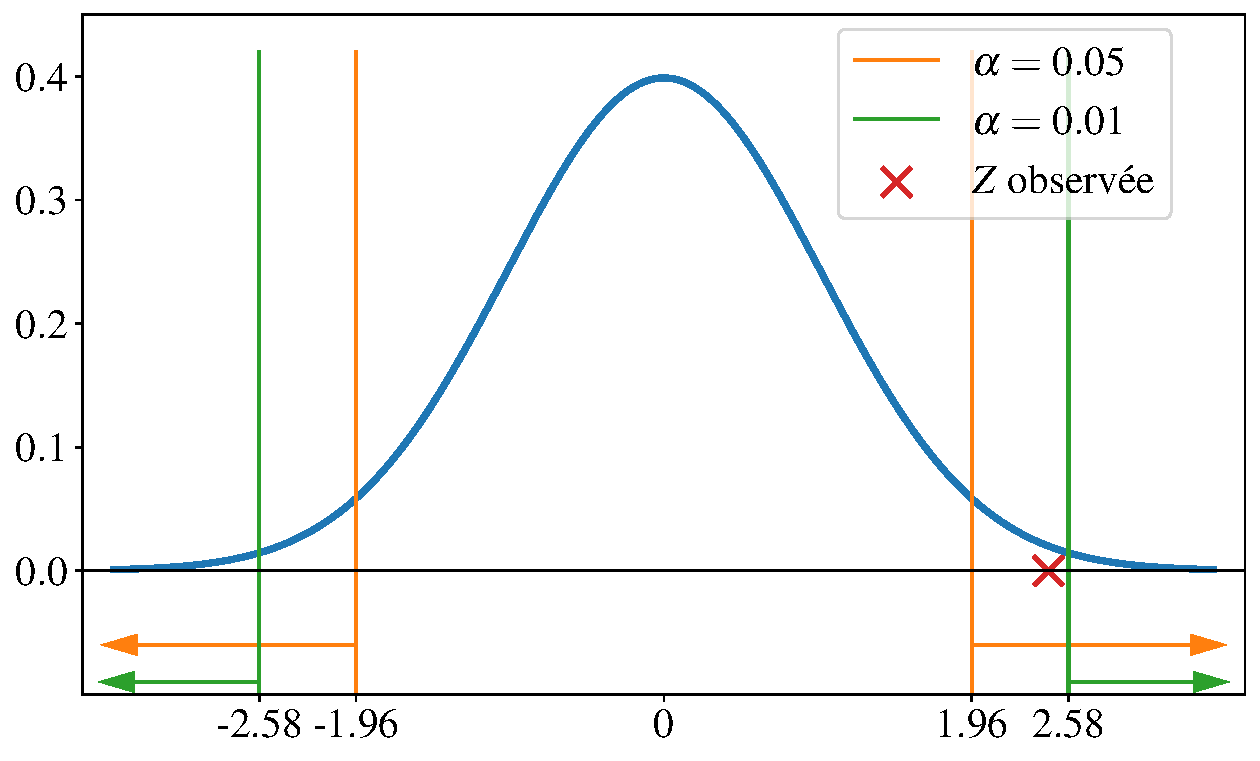
\includegraphics[width=0.65\textwidth]{figures/tests/z_pigeons}
  \caption{Densité d'une gaussienne centrée réduite. La valeur $z=2,45$ est
    dans le domaine de rejet pour $\alpha = 0,05$ mais pas pour
    $\alpha = 0,01$.}
  \label{fig:z_pigeons}
\end{figure}

\subsection{p-valeur}
\paragraph{Question :} Quelle est la p-valeur correspondant à la valeur de test
$z=2,45$ ?
\begin{answer}
  La p-valeur est
  \[
    \PP(\abs{Z} \geq \abs{z}) = \PP(Z \leq -\abs{z}) + \PP(Z \geq \abs{z}) = 2
    \PP(Z \leq -\abs{z}) = 2 \Phi(-\abs{z}) = 0,018.
  \]
  où $\Phi$ est la fonction de répartition d'une gaussienne standard.

  Cette p-valeur est bien inférieure au seuil de signification $\alpha = 0,05$,
  mais supérieure au seuil de signification $\alpha = 0,01$.
\end{answer}

\subsection{Test unilatéral à droite}
Supposons maintenant que nous nous demandons si les pigeons du Jardin du
Luxembourg, qui nous semblent particulièrement bien nourris de restes des
sandwicheries environnantes, ne seraient pas plus lourds que la moyenne de
300g. Il s'agit maintenant de faire un test unilatéral à droite, pour lequel
\[
  \HH_1 : \mu > \mu_0.
\]

\paragraph{Question :} Comment cela transforme-t-il notre test d'hypothèse ?
\begin{answer}
  Le test statistique consiste maintenant à rejeter $\HH_0$ si $Z > z_r$ (sans
  valeur absolue). En particulier, toutes les valeurs négatives nous font
  accepter $\HH_0$, contrairement au cas bilatéral.
  
  La valeur critique $z_r$ est telle que 
  \[
    \PP(Z > z_r) = \alpha, \text{ sachant } Z \sim \Ncal(0, 1).
  \]
  La densité de $Z$ étant symmétrique, on cherche donc $z_0$ telle que 
  \[
    \Phi(-z_r) = \alpha.
  \]
  
  Pour $\alpha = 0,05,$ la valeur critique est $z_r = 1,64.$ Pour
  $\alpha = 0,01,$ la valeur critique est $z_r = 2,33.$ L'hypothèse nulle est
  rejetée dans les deux cas.

  Le test unilatéral est plus puissant pour les valeurs du bon côté.

  Cet exemple est illustré sur la figure~\ref{fig:z_pigeons_unilateral}.
\end{answer}


\begin{figure}[h]
  \centering
  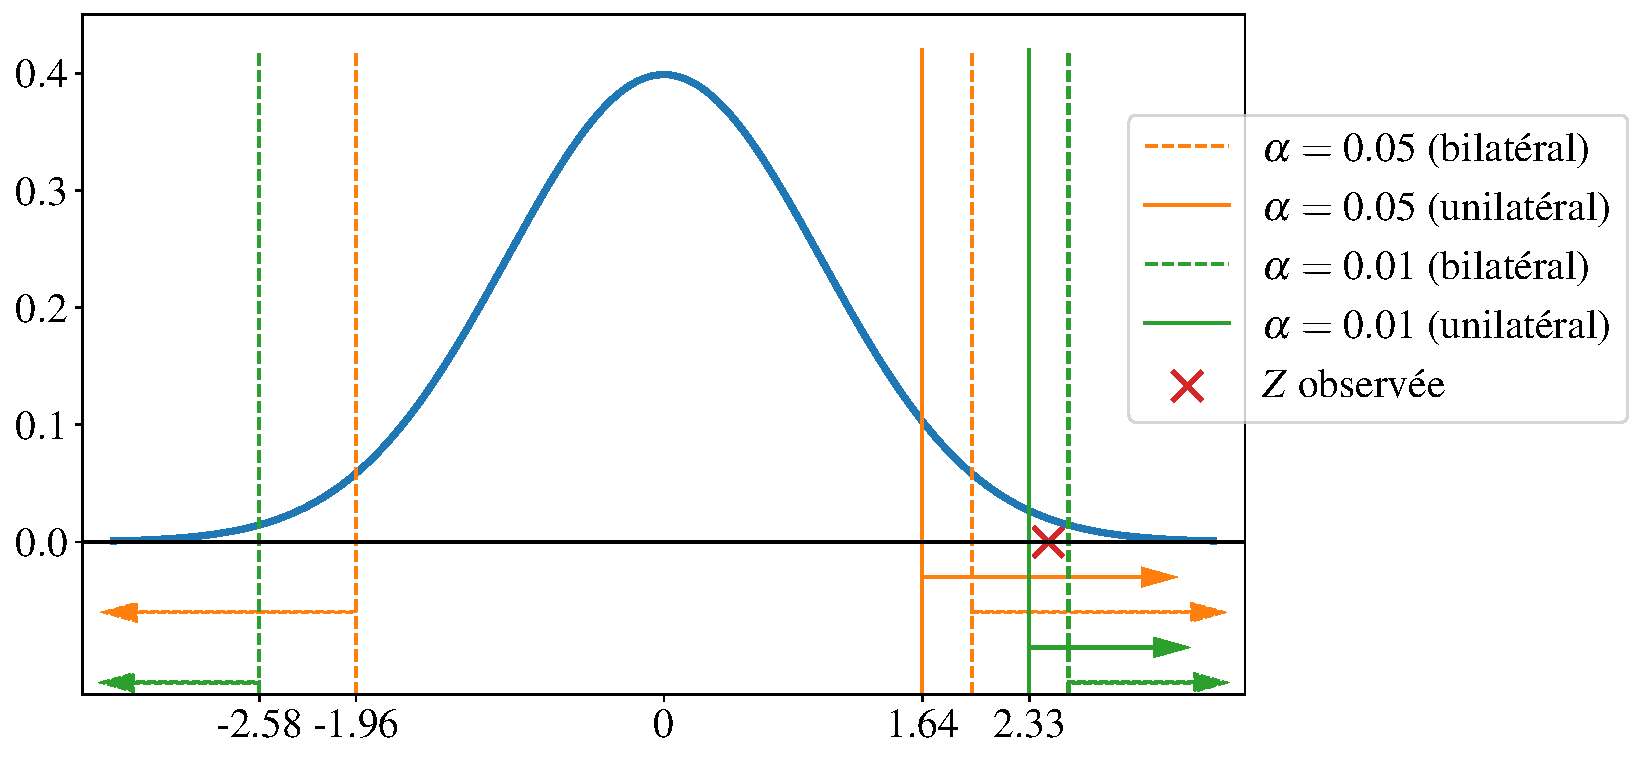
\includegraphics[width=0.85\textwidth]{figures/tests/z_pigeons_unilateral}
  \caption{Densité d'une gaussienne centrée réduite. La valeur $z=2,45$ est
    dans le domaine de rejet pour $\alpha = 0,05$ et pour $\alpha = 0,01$ dans
    le cas du test unilatéral.}
  \label{fig:z_pigeons_unilateral}
\end{figure}

\subsection{Intervalle de confiance $\bullet$}
\label{sec:ic}
Reprenons le test bilatéral.

Étant donné $\alpha,$ nous avons déterminé $z_0$ de sorte à ce que
\[
  \PP(\abs{Z} > z_0) = \alpha, \text{ sachant } Z \sim \Ncal(0, 1).
\]

En d'autres termes, 
\[
  \PP(-z_0 \leq Z \leq z_0) = 1 - \alpha. 
\]
(On pourra se référer à la figure~\ref{fig:z_moyenne}.)

D'après la définition de $Z$ (équation~\eqref{eq:z_moyennes}), cela est équivalent à 
\[
  \PP\left( M_n - \frac{\hatsigma}{\sqrt{n}} z_0 \leq 
    \mu \leq M_n + \frac{\hatsigma}{\sqrt{n}}z_0 \right) = 1 - \alpha.
\]

Ainsi l'intervalle 
\[
  \left[ M_n - \frac{\hatsigma}{\sqrt{n}} z_0, \; M_n +
    \frac{\hatsigma}{\sqrt{n}} z_0 \right]
\]
est un \textbf{intervalle de confiance} à $(1 - \alpha)$ pour la taille moyenne
$\mu$ (voir Probabilités V).

Dans notre exemple, l'intervalle de confiance à 95\% pour la valeur moyenne du
poids d'un pigeon est $[302,4\si{g}~; 321,6\si{g}]$.
$\mu_0 = 300\si{g}$ n'est pas dans l'intervalle de confiance ; on adopte l'hypothèse
alternative selon laquelle $\mu \neq \mu_0.$

L'intervalle de confiance à 99\% est $[299,4\si{g}~; 324,6\si{g}].$ Cet
intervalle contient $\mu_0$. On ne peut pas rejeter l'hypothèse nulle.

\paragraph{Exercice :} Calculer l'intervalle de confiance à 95\% et à 99\% pour
le test d'hypothèse unilatéral à droite. (Solution : cf section~\ref{sec:ic_sol}.)
% \section{Test d'indépendance du $\chi^2$}
% \label{sec:chi2}

\subsection{Tests de comparaison de moyenne $\bullet \bullet$} 
Le test que nous avons étudié dans cette section, qui permet de comparer la
moyenne d'un échantillon suffisamment large pour être dans la limite du
théorème centrale limite ($n \geq 30$) à sa moyenne théorique, s'appelle un
\textbf{test Z}, ou \textit{Z-test} en anglais, par référence à la notation $Z$
couramment utilisée pour une variable normalement distribuée de moyenne 0 et
variance 1.

Dans le cas d'un échantillon de faible taille, le théorème central limite ne
s'applique pas. Si l'on suppose $X$ normalement distribuée, on peut alors
appliquer un test de Student, ou test t (\textit{t-test} en anglais), ainsi
appelé car la statistique de test suit une loi de Student.

Des variantes de ces tests Z et t peuvent aussi être utilisés pour comparer les
moyennes de deux échantillons, appariés ou non. Deux échantillons aléatoires
$(X_1, X_2, \dots, X_n)$ et $(Y_1, Y_2, \dots, Y_n)$ sont dit appariés quand
les variables $X_i$ et $Y_i$ décrivent le même individu $i$. Il peut par
exemple s'agir de mesures répétées sur les mêmes individus, soit prises par
deux appareils différents, soit prises avant et après un traitement.



\section{Tests d'hypothèses multiples}
\label{sec:mht}
\paragraph{Question} Imaginons l'expérience de pile ou face suivante : je lance
15 fois une pièce équilibrée, et demande à Alice, qui est assise en face de
moi, de prédire avant chaque lancer si je vais obtenir pile ou face. Supposons
qu'Alice me donne la bonne réponse 12 fois. A-t-elle un don de
voyance ?
\begin{answer}
  Pour répondre à cette question, posons $X$ une variable de Bernouilli de
  paramètre $p$ modélisant, pour un lancer de pièce, le succès d'Alice :
  $X$ vaut 0 si Alice n'a pas donné la bonne prédiction et 1
  sinon. L'hypothèse nulle est
  \[
    \HH_o : p = 0,5 \text{ (Alice n'a pas de don de voyance)}.
  \]
  Nous pouvons ici poser une hypothèse alternative unilatérale à droite :
  \[
    \HH_1 : p > 0,5 \text{ (Alice a un don de voyance)}.
  \]
  Il s'agit du test binomial que nous avons défini dans la
  section~\ref{sec:formalisme_test}, mais ici la variable modélise non pas le
  résultat du lancer de pièce mais le statut (correct ou non) de la réponse
  donnée par Alice.

  La statistique de test $T$ est le nombre de succès dans l'échantillon. Sous
  $\HH_0$, $T \sim \Bcal(n, p).$ La p-valeur correspondant à 12 succès est donc
  $\PP_{\HH_0}(T \geq 12) = 1 - \PP(T \leq 11) = 0,018$. Cette p-valeur est
  significative pour $\alpha = 5\%$.
\end{answer}

\paragraph{Question} Supposons maintenant que je fasse ce test avec toute la
classe (sans communication entre les élèves). Trois élèves passent mon test de
pyschisme, autrement dit tombent juste au moins 12 fois sur 15. Dois-je appeler
la presse ?
\begin{answer}
  Supposons une promo de $m=127$ élèves. Nous posons maintenant $Y$ une
  variable de Bernouilli de paramètre $\pi$ modélisant le succès d'une personne
  sur 15 lancers. Nous faisons ici un nouveau test statistique sur $Y$,
  \[
    \HH_0^\prime : \pi = 0,018 \text { \qquad et \qquad} \HH_1^\prime : \pi >
    0,018.
  \]
  Il s'agit toujours d'un test binomial. La statistique de test $U$ est le
  nombre d'élèves passant le test. Sous $\HH_0^\prime$, $U \sim \Bcal(m,
  \pi)$.
  La p-valeur est ici
  $\PP_{\HH_0^\prime}(T \geq 3) = 1 - \PP(T \leq 2) = 0,40.$ Cette p-valeur
  n'est pas significative !
\end{answer}

Cet exemple illustre le principe suivant : plus on fait de tests, et plus on a
de chances de voir apparaître une p-valeur significative. 

Il est nécessaire de corriger cet effet : on parle de \textbf{correction} ou
\textbf{ajustement de tests d'hypothèse multiples.} La plus simple et plus
utilisées de ces corrections, proposée par la biostatisticienne Olive Jean
Dunn, est connue sous le nom de \textbf{correction de Bonferroni} : il s'agit
simplement de diviser le niveau de signification par le nombre de tests
\[
  \alpha \leftarrow \frac{\alpha}{m}.
\]

Cette correction se justifie de la façon suivante : notons
$p_1, p_2, \dots, p_m$ les p-valeurs obtenue pour $m$ tests, testant chacun
$\HH_0$ vs. $\HH_1$, et supposons que $\HH_0$ est vraie pour les $m_0$ premiers
tests. Alors la probabilité de rejeter au moins une de ces hypothèses nulles est
\[
  \PP\left(\bigcup_{i=1}^{m_0} \left( p_i \leq \frac{\alpha}{m} \right)\right)  \leq
  \sum_{i=1}^{m_0} \PP \left( p_i \leq \frac{\alpha}{m} \right)= \frac{m_0
    \alpha}{m} \leq \alpha.
\]



% \section{Compléments}
\section{Solution de l'exercice section~\ref{sec:ic} $\bullet$}
\label{sec:ic_sol}
Nous avons déterminé la valeur critique $z_r$ de sorte à ce que 
  \[
    \PP(Z \leq z_r) = 1-\alpha.
  \]

Comme $Z = \frac{\sqrt{n} (M_n - \mu_0)}{\hatsigma}$, cela est équivalent à 
\[
  \PP \left(\mu \geq M_n - \frac{\hatsigma}{\sqrt{n}} z_r \right) = 1 - \alpha.
\]

Ainsi l'intervalle 
\[
  \left[M_n - \frac{\hatsigma}{\sqrt{n}} z_r, +\infty \right]
\]
 est un intervalle de confiance unilatéral à $(1-\alpha)$ pour la taille moyenne $\mu$.

 Dans notre exemple, l'intervalle de confiance unilatéral à droite à 95\% pour
 la valeur moyenne du poids d'un pigeon est $[303,9\si{g}, +\infty]$. Cet
 intervalle contient $\mu_0$ et on ne peut pas rejeter l'hypothèse nulle.  À
 99\%, cet intervalle est $[300,6\si{g}, +\infty[.$ Ces résultats sont
 cohérents.

\begin{plusloin}
\item On dit d'un test statistique qu'il est sans biais si sa puissance est
  supérieure au niveau de signification : $1 - \beta > \alpha$.
\item On dit d'un test statistique qu'il converge si la suite des erreurs de
  deuxième espèce converge vers $0$ : $1 - \beta \cvn 0.$ 
\item Pour plus de détails sur la sur-interprétation des p-valeurs en sciences
  et le \textit{p-hacking} (consistant à ne conserver, parmi de nombreux tests
  conduits sur les données, ceux qui donnent des p-valeurs significatives), on
  pourra se reporter aux références suivantes.
  \begin{thebibliography}{99}
  \bibitem{ioannidis2005}
    John PA Ioannidis.
    {Why most published research findings are false.}
    \textit{PLoS medicine,} 
    2(8):{e124},
    {2005.}

  \bibitem{head2015}
    Megan L Head, Luke Holman, Rob Lanfear, Andrew T Kahn and Michael D Jennions.
    {The extent and consequences of p-hacking in science.}
    \textit{PLoS biology},
    13(3):{e1002106},
    {2015.}
  \bibitem{wasserstein2016}
    Ronald L Wasserstein, Nicole A Lazar, et al.
    {The ASA's statement on p-values: context, process, and purpose}.
    \textit{The American Statistician},
    70(2):129--133,
    2016.

  \bibitem{holmes2018}
    Susan Holmes.
    {Statistical proof? The problem of irreproducibility}.
    \textit{Bulletin (New Series) of the American Mathematical Society},
    {55}(1), 2018.
  \end{thebibliography}
\end{plusloin}

%-*- coding: utf-8 -*-
\section{QCM}

\paragraph{Question 1.} Dans une étude dont le but est de déterminer si la
consommation de chocolat noir améliore les résultats scolaires, l'hypothèse
alternative est :
\begin{itemize}
\item[$\square$] Les élèves qui consomment du chocolat noir obtiennent les
  mêmes résultats que les élèves qui n'en consomment pas.
\item[$\square$] Les élèves qui consomment du chocolat noir obtiennent de moins
  bons résultats que les élèves qui n'en consomment pas.
\item[$\square$] Les élèves qui consomment du chocolat noir obtiennent de
  meilleurs résultats que les élèves qui n'en consomment pas.
\item[$\square$] Les élèves qui consomment du chocolat noir obtiennent des
  résultats différents des élèves qui n'en consomment pas.
\end{itemize}

\paragraph{Question 2.} La p-valeur est :
\begin{itemize}
\item[$\square$] La probabilité que l'hypothèse nulle soit vraie.
\item[$\square$] La probabilité que l'hypothèse alternative soit vraie.
\item[$\square$] La probabilité, si l'hypothèse nulle est vraie, d'obtenir une
  situation au moins aussi surprenante que celle observée.
\item[$\square$] La probabilité, si l'hypothèse alternative est vraie,
  d'obtenir une situation au moins aussi surprenante que celle observée.
\end{itemize}

\section*{Solution}
{%
\noindent
\rotatebox[origin=c]{180}{%
\noindent
\begin{minipage}[t]{\linewidth}
\paragraph{Question 1.}
L'hypothèse alternative est que les élèves qui consomment du chocolat noir
obtiennent de meilleurs résultats que les élèves qui n'en consomment pas. Il
s'agit d'un test unilatéral. Le test sera plus puissant que si on utilise
l'hypothèse alternative bilatérale (les résultats entre les deux groupes sont
différents). Cependant, si ce test unilatéral ne permet pas de rejeter
l'hypothèse nulle, il sera impossible de déterminer si c'est parce qu'il n'y a
pas de différence entre les deux groupes ou parce que l'effet est dans l'autre
sens.

Remarquons enfin que corrélation n'est pas causalité : ce test permet de
déterminer si la différence de performance entre les élèves cacaophiles et les
autres est significative, mais en aucun cas si elle est \textit{due} à la
consommation de chocolat. Il est tout à fait possible que la consommation de
chocolat noir soit liée à d'autres facteurs (en particulier sociaux) qui eux
influent sur la réussite scolaire. \newline

\paragraph{Question 2.} La p-valeur est la probabilité d'obtenir une situation
au moins aussi surprenante que celle observée si l'hypothèse nulle est
vraie. Il est très important de ne pas l'interpréter comme la probabilité que
l'hypothèse nulle soit vraie : 
\[
  \PP(t \geq t_0 | \HH_0) \neq \PP(\HH_0 | t \geq t_0). 
\]
\end{minipage}%
}%

%%% Local Variables:
%%% mode: latex
%%% TeX-master: "../../sdd_2025_poly"
%%% End:


%%% Local Variables:
%%% mode: latex
%%% TeX-master: "../sdd_2025_poly"
%%% End:


